\documentclass[a4paper,12pt]{article}
\usepackage[utf8]{inputenc}
\usepackage{wrapfig}
\usepackage{graphicx}
\usepackage{float}
\usepackage{amsmath}
\usepackage{pslatex}
\usepackage[portuguese]{babel}
\usepackage{indentfirst}
\usepackage{tikz}
\usepackage[lmargin=3cm,rmargin=3cm,tmargin=2.5cm,bmargin=2.5cm]{geometry}
\setlength{\parindent}{1cm}
\setlength{\baselineskip}{1.5cm}
\renewcommand{\contentsname}{Sumário}



\begin{document}

\begin{titlepage}
 \begin{center}
  { \large FUNDAÇÃO GETULIO VARGAS}\\[0.3cm]
  { \large ESCOLA DE MATEMÁTICA APLICADA}\\[0.5cm]
  { \large CURSO DE GRADUAÇÃO EM}\\[0.3cm]
  { \large MATEMÁTICA APLICADA}\\[0.3cm]
 
  \vspace{55 mm}

  {\bf \large Dinâmica de Disseminação de Notícias em}\\[0.1cm]
  {\bf \large Redes Complexas}\\[1.7cm]

  { por}\\[0.6cm]
  {\large Elisa Mussumeci}\\[0.1cm]


  \vspace{7cm}

  { Rio de Janeiro}\\[0.1cm]
  { 2015}\\[0.6cm]
  { FUNDAÇÃO GETÚLIO}\\[0.1cm]
  { VARGAS}\\[0.1cm]
 \end{center}
\end{titlepage}

\begin{titlepage}
 
 \begin{center}
  {\large FUNDAÇÃO GETULIO VARGAS}\\[0.3cm]
  {\large ESCOLA DE MATEMÁTICA APLICADA}\\[0.5cm]
  {\large CURSO DE GRADUAÇÃO EM}\\[0.3cm]
  {\large MATEMÁTICA APLICADA}\\[0.3cm]


  \vspace{20 mm}


  {\large Dinâmica de Disseminação de Notícias em}\\[0.1cm]
  {\large Redes Complexas}\\[2.5cm]

  
  \bf "Declaro ser o único autor do presente projeto de monografia que refere-se ao
plano de trabalho a ser executado para continuidade da monografia e ressalto
que não recorri a qualquer forma de colaboração ou auxílio de terceiros para
realizá-lo a não ser nos casos e para os fins autorizados pelo professor orientador"

  \vspace{3.5cm}


  \line(1,0){220}\\[0.1cm]
  {\bf Elisa Mussumeci}\\[2cm]
  {\bf Orientador: Flavio Codeço Coelho}\\[5cm]




  {Rio de Janeiro}\\[0.1cm]
  {2015}
 \end{center}
\end{titlepage}

\begin{titlepage}
 \begin{center}
 
  {\bf \large ELISA MUSSUMECI}\\[0.3cm]

  \vspace{25 mm}

  {\bf \large Dinâmica de Disseminação de Notícias em}\\[0.1cm]
  {\bf \large Redes Complexas}\\[4cm]

  {“Monografia apresentada à Escola de Matemática Aplicada}\\[0.1cm]
  {como requisito parcial para obtenção do grau de Bacharel }\\[0.1cm]
  {em Matemática Aplicada”}\\[6cm]


  {Aprovado em \ \line(1,0){20} \ \ de \line(1,0){62} \ \ de \line(1,0){30} \ .}\\[0.1cm]
  {Grau atribuido ao Projeto de Monografia: \line(1,0){20} \ . }\\[3cm]
  
  
  {\line(1,0){250}}\\
  {\bf Professor Orientador: Flavio Codeço Coelho}\\[0.1cm]
  {\bf Escola de Matemática Aplicada}\\[0.1cm]
  {\bf Fundação Getulio Vargas}
 \end{center}
\end{titlepage}

\newpage\null\thispagestyle{empty}\newpage

\tableofcontents

\pagebreak

\begin{abstract}
 
O processo de formação de opinião é fortemente influenciado pela mídia digital.
Entretanto pouco se sabe sobre o processo de disseminação de notícias e os fatores que determinam o alcance de cada
notícia.

A disseminação de uma notícia se dá por meio de um ou mais caminhos em uma rede desconhecida de influência entre 
formadores de opinião (produtores de notícias). Este padrão pode ser recuperado, com algum grau de incerteza, a partir de dados
da sequência temporal das publicações sobre um mesmo tema, e dos links nelas contidos.

Este projeto tem como objetivo caracterizar as redes de interligação de veículos de mídia e modelar a dinâmica do espalhamento 
de notícias, a fim de prever tendências e mapear questões de interesse.

\end{abstract}

\pagebreak


\section{Introdução}

\section{Metodologia}

\subsection{Dados Utilizados}

Para a realização deste trabalho, foram utilizados os dados do projeto MediaCloud Brasil. O MediaCloud Brasil é um projeto concebido e mantido pelo
NAMD/EMAp da Fundação Getúlio Vargas, e vem ao longo dos últimos três anos monitorando mais de cem mil veículos de mídia da internet brasileira. Possui em
sua base de dados mais de um milhão de artigos capturados.

O projeto utiliza como banco de dados o MongoDB, um banco de dados de documentos open-source de alta performance. O MongoDB é classificado como um banco de 
dados 'NoSQL', uma vez que evita a tradicional estrutura  baseada em tabela relacional e utiliza documentos JSON com esquemas dinâmicos para armazenamento 
dos documentos. A vantagem de utilizar o JSON é realizar a integração de dados em certos tipos de aplicações de forma mais fácil e mais rápida.

\subsubsection{Escolha de uma Notícia}

Para analisar a dinâmica de disseminação de notícias na mídia brasileira, escolhemos notícias e acompanhamos o seu comportamento no decorrer 
do tempo.
Entretanto, o processo de escolha dessas notícias não é trivial, visto que determinar se um artigo fala sobre determinado assunto requer
uma análise elaborada de cada artigo.

Para contornar esse problema inicialmente, escolhemos notícias que surgiram na mídia apenas relacionadas a um assunto, como por exemplo o atentado
do Charlie Hebdo, Rolezinhos, etcs.

No decorrer deste trabalho utilizaremos como exemplo para análises os dados referentes ao atentado ao Charlie Hebdo.
  
\subsubsection{Estatísticas Básicas}

No banco de dados do MediaCloud, pudemos observar 2136 artigos referentes ao Charlie Hebdo. Abaixo temos um gráfico desses artigos
no tempo:

\begin{figure}[h]
 \centering
 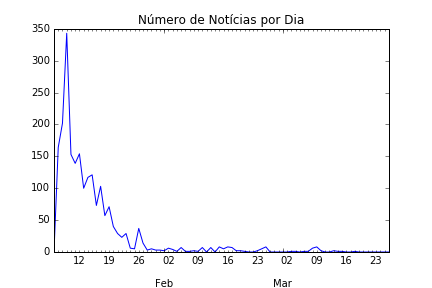
\includegraphics[scale=0.7]{../grafic.png}
 % grafic.png: 432x288 pixel, 72dpi, 15.24x10.16 cm, bb=0 0 432 288
\end{figure}


  \pagebreak
\subsection{Recuperação de Informação}

  Ao estudar e analisar um conjunto de textos, precisamos traduzi-lo para uma linguagem computacional de forma que possamos aplicar modelos e heurísticas 
  conhecidas para extrair informação dele. Esse processo é chamado de \textit{Recuperação da Informação} (RI).
    
  
\subsubsection{Modelos Utilizados}

  Na realização do processo de RI, utilizamos dois modelos: Word2Vec e Tf-Idf
  
  O modelo \textbf{Tf-Idf}, (\textit{term frequency-inverse document frequency}), é uma medida estatística que tem o intuito de indicar
  a importância de uma palavra de um documento em relação a um corpus linguístico muito usada para rankeamento de documentos em uma consulta. O Tf-Idf trata-se do produto entre as estatísticas $Tf_{d,t}$ e
  $Idf_{t}$.
  
  Dado um conjunto de $N$ documentos, $Tf_{d,t}$ é a frequência do termo $t$ no documento
  $d$, ou seja, o número de vezes em que $t$ ocorre em $d$. Usamos o termo $Tf$ para computar escores de correspondência consulta-documento,
  porém, o $Tf$ nos dá a frequência absoluta dos termos, o que faz com que um termo que possua $Tf=10$ seja 10 vezes mais relevante do um que possua
  $Tf=1$. 
  
  Podemos concordar que um documento com $Tf=10$ é mais relevante do que um com $Tf=1$, porém não necessariamente 10 vezes mais relevante.
  A relevância não aumenta em proporção com a frequência do termo. Para contornar isso, é comum usar ao invés da frequência absoluta uma ponderação
  pelo $Log$ da frequência. Dessa forma, o peso $log$ da frequência do termo $t$ em $d$ é definido como:
  
  $$W_{t,d}=\begin{cases}
             1 + logTf_{t,d}  \hspace{1cm} \text{se} \ Tf_{t,d} > 0 \\
             0 \ \hspace{3cm} \text{caso contrário}
            \end{cases}
 $$
 
 
 Exemplificamos abaixo a correspondência de valores $Tf_{t,d}$ absoluto com a ponderação $W_{t,d}$:
 
 \begin{center}
  \begin{tabular}{ll}
    \hline
    $Tf_{t,d}$ & $W_{t,d}$\\
    \hline
    0&0\\
    1&1\\
    2&1.3\\
    10&2\\
    1000&4\\
    
  \end{tabular}
 \end{center}
 
 
  Sabemos que nem todo termo frequente em um documento pode ser considerado muito relevante. Consideramos uma consulta com dois termos:
  um frequente no conjunto de documentos e outro raro. Não queremos que um documento que possua o termo frequente seja mais relevante do que o
  documento que possua o termo raro.

  Inferimos então que termos raros são mais informativos do que termos frequentes. Dessa forma, queremos dar uma maior relevância para
  termos raros do que para termos muito frequentes. Para incluir isso em nossa medida usamos o termo $Idf$.
  
  O termo $Idf_{t}$ é uma medida de informatividade do termo $t$, que afeta o rankeamento de documentos para consultas com pelo menos dois
  termos. Com ele aumentamos o peso relativo de termos raros e diminuimos o peso relativo
  de termos muito frequentes. O definimos da seguinte maneira:
  
  $$ Idf_{t}\ = \ log\ \frac{N}{df_{t}}$$
  
  Onde $df_{t}$ é a frequência de documento, o número de documentos em que $t$ ocorre. Consideramos $df_{t}$ uma medida inversa da informatividade
  do termo $t$.
  
  Ao multiplicarmos o termo $Idf$ ao nosso peso ponderado $W_{t,d}$, temos a medida Tf-Idf. O peso Tf-Idf aumenta com o número de ocorrências
  dentro de um documento e com a raridade do termo na coleção. É considerado o melhor esquema de ponderação em recuperação da informação.
  
  $$ W_{t,d} = (1 + log Tf_{t,d}) \cdot \ log \dfrac{N}{Df_{t}}$$
  
    
  
\subsubsection{Representação Artigos}

  Para criarmos o modelo Word2Vec, fornecemos como entrada um corpus linguístico (coleção de documentos) e o modelo nos retorna uma matriz
  onde cada palavra é representada por um vetor. Podemos ver a seguir a matriz resultante desse modelo em nosso conjunto de dados:
  
  $$\begin{bmatrix}
     -1.13546148e-01 & -8.23762193e-02 & ... & -1.48673728e-01\\
     -7.33665004e-02 &  1.13490485e-01 & ... &  1.01513676e-01\\
     -1.17934421e-02 & 1.34973019e-01  & ... &  1.22169554e-02\\
     ... & & &  \\
     -1.04698418e-02 & 4.16711420e-02 & ... &  1.23268731e-01\\
      1.67298820e-02 &   4.50479165e-02 & ... & -1.80342391e-01\\
     -3.84105071e-02 &   7.35700727e-02 & ... &  4.78151329e-02
    \end{bmatrix}
 $$
 
  Temos nessa matriz a representação de todas as palavras presentes em nosso corpus, porém, queremos representar documentos e não palavras.
  Para isso, buscamos o vetor referente de cada palavra contida em um documento e somamo-os. Dessa forma, associamos todas as palavras contidas
  em um documento, e transformamo-as em um único vetor. Ou seja, dado um documento A, sabemos que ele é composto pelo seguinte conjunto de palavras
  $P:\{1,2,3,4,5\}$. Para cada termo buscamos o seu vetor representativo $v_{t}$, $t =\{1,2,3,4,5\}$ e somamos todos esses vetores, criando o vetor
  $v_{d}$ que representa o vetor do documento D:
  
  $$v_{d} = v_{1}+v_{2}+v_{3}+v_{4}+v_{5} $$
  
  Representando um documento dessa forma, não levamos em consideração a importância de cada palavra para o documento, o que nos faz ter
  uma representação pouco eficiênte. Para contornar isso, iremos antes de somar os vetores referentes às palavras, multiplicá-los 
  pelo valor TF-IDF de cada palavra em cada documento. Dessa forma temos para cada palavra um valor $w_{t,d}$, $i=\{1,2,3,4,5\}$ referente
  ao valor TF-IDF to termo $t$ no ducumento $d$:
  
  $$v_{D} = \sum_{i=1}^{5} v_{i} \cdot w_{t,d} $$


\subsection{Rede de Disseminação}
 
 Um dos desafios da área de epidemiologia é como representar dinâmicas de disseminação de doenças. Uma representação muito comum que se tornou popular após o modelo
 do mundo pequeno (adicionar referência), foi a modelagem através de Redes Complexas.
 
 O termo Redes Complexas se refere a um grafo que apresenta uma estrutura topográfica não trivial, composto por um conjunto
 de vértices (nós) que são interligados por meio de arestas (Barabási, 2003). A teoria das Redes Complexas  está relacionada com a modelagem de redes reais, através da 
 análise de dados empíricos. Redes Complexas não são estáticas (evoluem no tempo alterando sua estrutura), e 
 constituem estruturas onde processos dinâmicos (como disseminação de virus ou opiniões) podem ser simulados.
 
 Sendo assim, criamos uma rede complexa para representar a disseminação da notícia do Atentado ao Charlie Hebdo. Para construir a rede
 consideramos como contaminação sofrer influência de outro artigo, ou seja, um artigo A contamina um artigo B se o artigo A influenciou o
 artigo B.
 
 Dessa forma, em nossa rede, os vértices representam os artigos, e as arestas a relação de influência entre eles, isso é, dado um nó $e_{i}$ e um nó
 $e_{j}$ existe uma aresta $a_{ij}$ que sai de \textit{i} e vai para \textit{j} se o artigo \textit{i} influênciou o artigo \textit{j}.
 
 
 
 
\subsubsection{Definição de Influência}
 
 Para definir quando um artigo influencia outro em nossa rede, foram usadas duas heurísticas: similaridade de cosseno e temporalidade.
 
 A similaridade de cosseno utiliza da distância de cossenos para definir se dois artigos são similares ou não. A distância de cosseno
 consiste em calcular o cosseno entre o ângulo que os dois vetores formam. Podemos calculá-lo utilizando a fórmula abaixo:
 
 $$ cos(\theta) = \dfrac{A \cdot B}{\parallel A\parallel \parallel B \parallel} $$
 
 Caso a distância de cossenos entre os dois artigos for pequena, então os consideramos similares. Possuindo dois artigo similares, ainda não
 sabemos qual influênciou e qual foi o influenciado. Para definir essa questão, utilizamos a data e hora em que cada um foi publicado.
 
 Dessa forma, se dois artigos são similares, consideramos como influenciador aquele que foi publicado primeiro. Abaixo temos uma visualização da
 rede criada:

 \begin{figure}[h]
 \centering
 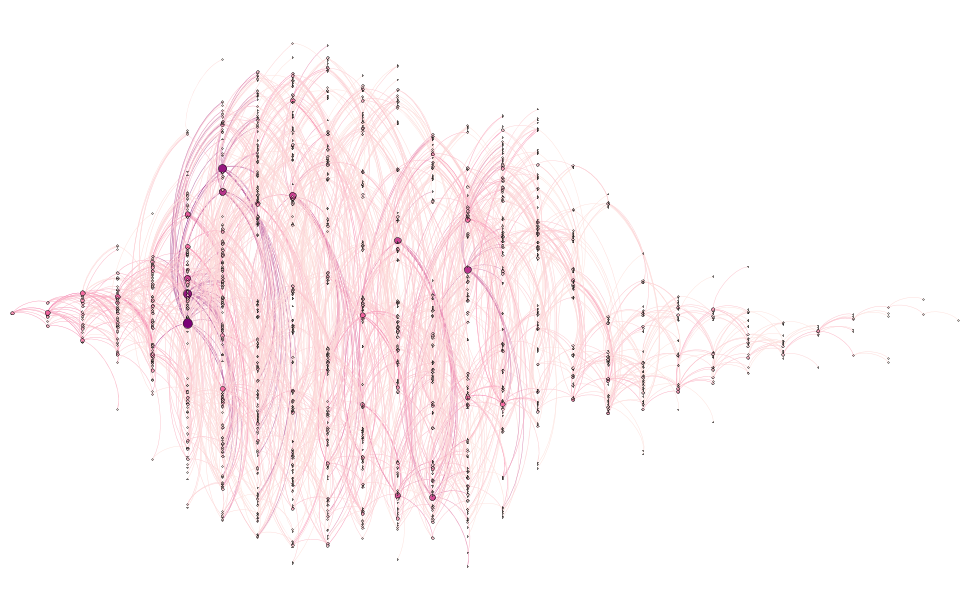
\includegraphics[scale=0.5]{../Untitled.png}
 % Untitled.png: 969x591 pixel, 72dpi, 34.18x20.85 cm, bb=0 0 969 591
\end{figure}



 
\subsubsection{Escolha de Limiares}

 Ao definir influência, consideramos que os artigos são similares se possuem uma distância de cosseno pequena. Porém, não definimos
 o quão pequena essa distância tem que ser. 
 
 Inicialmente foram utilizado valores escolhidos aleatóriamente, entretanto, essa não é a melhor forma de escolher esses valores.
 Sendo assim, serão feitas análises nas distribuições das distâncias para podermos encontrar limiares mais justos para a criação da rede.
 
 
\subsubsection{Análises}

 Nesta seção serão realizadas análises na rede de disseminação, como análisar os caminhos presentes na rede a partir de determinados veículos, análisar
 a distribuição dos caminhos da rede, observar o subgrafos presentes, entre outros.
 
\section{Resultados}
 
\subsection{Validação da Rede}

\subsection{Modelos Epidemiológicos}

\subsection{Validação da Rede de Disseminação}

\subsection{Modelo de Disseminação}

\subsection{Simulações}

\subsection{Comparação de Resultados}

\section{Conclusão}

\end{document}
